\documentclass[a4paper,english]{article}
\usepackage[T1]{fontenc}
\usepackage[latin1]{inputenc}
\usepackage{babel}
\usepackage{times}
\usepackage{epsfig}
\usepackage{geometry}

\newcommand{\til}{\raisebox{-1ex}{\~{}}}
\newcommand{\partner}[8]{
  \noindent\begin{tabular}{p{0.47\textwidth}p{0.47\textwidth}}
    \multicolumn{2}{l}{\textbf{#1}}\\
    \multicolumn{2}{l}{#2}\\
    \multicolumn{2}{l}{#3}\\
    #4 & #5\\
    E-mail: \texttt{#8}\\
    Phone: #6 & Fax: #7\\
  \end{tabular}\par
  \vspace{2ex}
}

\title{\textsc{Snow}: a Parallel Programming Environment\\ for Clusters
  of Workstations}

\author{}

\date{}

\begin{document}
\pagestyle{empty}

\maketitle
\thispagestyle{empty}

\section{Partners}

\subsection*{Academic Partners}

\partner{Prof. Dr. Wolfgang Schr�der-Preikschat} {Forschungszentrum
  Informationstechnik GmbH (GMD)} {Forschungsinstitut f�r
  Rechnerarchitektur und Softwaretechnik (FIRST)} {Kekul�strasse 7}
{12489 Berlin, Germany} {+49 30 6392-1841}{+49 30 6392-1805}
{wosch@first.gmd.de}{}

\partner{Prof. Dr. Philippe Olivier Alexandre Navaux} {Universidade Federal do Rio
  Grande do Sul (UFRGS)} {Instituto de Inform�tica (II)} {Av. Bento
  Gon�alves 9500} {91501-970 Porto Alegre, RS, Brazil} {+55 51
  316-6165}{+55 51 316-1576} {navaux@inf.ufrgs.br}

\partner{Prof. Ant�nio Augusto Medeiros Fr�hlich} {Universidade Federal de
  Santa Catarina (UFSC)} {Departamento de Inform�tica e de Estat�stica
  (INE)} {Campus Universit�rio Trindade, CP 476} {88049-900,
  Florian�polis, SC, Brazil} {+55 48 331-9498}{+55 48 331-9770}
{guto@inf.ufsc.br}

\partner{Prof. Dr. S�rgio Takeo Kofuji} {Universidade de S�o Paulo
  (USP)} {Laborat�rio de Sistemas Integr�veis (LSI)} {Av. Prof. Luciano
  Gualberto, 158, CP8174} {05508-900, S�o Paulo, SP, Brazil} {+55 11
  818-5667}{+55 11 211-4574} {kofuji@lsi.usp.br}

\subsection*{Industrial Partners}

\partner{Dr. Hans-Georg Paap} {GENIAS Software GmbH} {Computational
  Fluid Dynamics} {Erzgebirgstrasse 2} {93073 Neutraubling, Germany}
{+49 9401 9200-30}{+49 9401 9200-92} {hgp@genias.de}

\partner{Eng. Luiz Francisco Gerbase} {ALTUS Sistemas de Inform�tica
  Ltda} {Departamento de Automa��o Industrial} {Av. S�o Paulo, 555}
{90230-161, Porto Alegre, RS, Brazil} {+55 51 337-3633}{+55 51 337-3632}
{altus@altus.com.br}


\section{Motivation}

The parallel computing community has been using clusters of commodity
workstations as an alternative to expensive massively parallel
processors (MPP) for several years. While MPPs can rely on custom
hardware to achieve high performance, their development follows a slow
pace, mainly due to the small production scale. Clusters, in the other
hand, benefit from the frenetic pace with which the workstation market
evolves. As a matter of fact, when an MPP comes to the market, it is
very likely that processor, memory and interconnection systems with
similar features will already be available at the commodity market.
Therefore, it seems evident that both technologies are going to converge
into a single one.

However, when we compare the performance of parallel applications
running on clusters and on MPPs, the figures show a quite different
scenario: clusters are still far behind their expensive relatives. The
Numerical Aerospace Simulation Facility from NASA has carried out a
careful study on parallel computing performance. This study, better
known as the NAS Parallel Benchmark, corroborates the superiority of
MPPs.

Taking in consideration these two observations, we concluded that the
gap between MPPs and clusters has its origin in the parallel programming
software environment normally used in clusters. While MPPs rely on
custom software specifically developed to support parallel applications
on a given parallel architecture, clusters often apply the ``commodity''
principle also to the software. Commodity workstation software, however,
has not been designed to support parallel computing.


\section{Objectives}

In this project, we intend to develop a comprehensive programming
environment to support parallel computing on clusters of commodity
workstations. This software environment shall include a parallel
language and a run-time system to support the development of high
performance parallel applications. In order to enable existing
application to run on the proposed environment, it shall also support
traditional standard interfaces from the parallel community, such as
\textsc{Posix} and MPI. Visual tools to configure and manage the
environment shall also be considered. Each of these goals will be
briefly discussed below.

\begin{itemize}
\item \textbf{Run-time support system:} cluster resources, e.g.
  processor time, storage area, and communication channels, shall be
  made available to parallel applications through a highly scalable
  run-time support system. This system shall support reconfigurations as
  to satisfy the requirements of particular parallel applications, yet
  delivering the expected
  performance~\cite{Froehlich:sbac:1999}~\cite{Schoen:1998}. The aimed
  run-time system shall also contemplate parallel operations such as
  group communication and collective
  operations~\cite{Barreto:1998}~\cite{Barreto:2000a}.
  
\item \textbf{Standard interfaces:} many existing parallel applications
  have been written considering standard interfaces. Independently from
  the development methodology and the programming environment adopted,
  most of these applications rely, in their lowest levels, on some
  subset of \textsc{Posix} system calls to access local resources, and
  on some inter-node communication package, typically MPI. Thereafter,
  these two interfaces shall be supported by our run-time support system
  in order to bring several existing parallel applications to run in
  \textsc{Snow}~\cite{Horta:1998}\cite{Torres:1997}. Nevertheless, only
  the interfaces shall be ported, not their traditional implementations.
  
\item \textbf{Parallel programming language:} writing parallel
  applications using standard sequential languages enriched with
  communication libraries is not always adequate. Adopting a parallel
  language eases the application development at the same time it
  increases performance due to better resource utilization. Moreover,
  some optimizations are only possible when the compiler is aware of
  application parallelism. Thus, \textsc{Snow} shall include a parallel
  programming language, offering a suitable mechanism to explore both
  fine and medium-grain concurrency. As to reduce the impact of a new
  language, our parallel language shall be a C++ extension, opening the
  way for distributed and parallel objects~\cite{Cavalheiro:1993}.
  
\item \textbf{Management tools:} one of the most serious problems in a
  cluster environment is to keep all the paraphernalia working. Noise,
  heat, and a confusing set of wires are normal when ``commodity'' is
  involved. Since avoiding this is not possible, we will work to make
  this ``chaos'' manageable with a set of tools, which shall implement a
  central management console with a friendly graphical interface for
  \textsc{Snow}~\cite{Bernal:1999}.

\item \textbf{Parallel and embedded applications:} a parallel
  programming environment is of no value if parallel applications cannot
  benefit of it. In oder to validate our environment, we intend to port
  and develop real parallel applications to run on it. Both of our
  industrial partners shall collaborate intensively with the
  requirements specification and design of our platform development, in
  such a way as to grant that \textsc{Snow} will find its way through
  real applications. Aimed application areas are computational fluid
  dynamics (GENIAS) and parallel embedded systems to control complex
  industrial processes (ALTUS).
\end{itemize}


\section{Work plan}

We believe we can achieve a parallel programming environment that
matches the goals described above by merging our current researches.
Each of the partners involved in this project is currently working is
some particular aspect of the proposed parallel programming environment,
however, our current research projects show small intersections. The
activities that have to be carried out in order to achieve the proposed
parallel programming environment are summarized in table
\ref{tab:tasks}, along with a time schedule and a task distribution
sketch.

\begin{center}
  \begin{table}[htbp]
    \begin{tabular}{cll}
      \textbf{Period}&\textbf{Activity}&\textbf{Partners}\\
      \hline 
      &\textbf{1 - Requirement analysis and definition of protocols}&\\
      &1.1 - to give the run-time support system an MPI adaption layer&\small{GMD, UFSC, USP}\\
      \textbf{4/2001}&1.2 - to give the run-time support system a \textsc{Posix} adaption layer&\small{GMD, UFSC, UFRGS}\\
      till&1.3 - to integrate the run-time support into the environment&\small{GMD, UFSC}\\
      \textbf{9/2001}&1.4 - to integrate the parallel language into the environment&\small{UFRGS}\\
      &1.5 - to integrate the management tools with the environment&\small{USP}\\
      &1.6 - to integrate the applications with the environment&\small{GENIAS, ALTUS}\\
      \hline
      &\textbf{2 - Parallel programming environment development}&\\
      &2.1 - run-time support system&\small{GMD, UFSC}\\
      \textbf{10/2001}&2.2 - MPI adaption layer for the run-time support system&\small{UFSC, USP}\\
      till&2.3 - \textsc{Posix} adaption layer for the run-time support system&\small{UFSC, UFRGS}\\
      \textbf{3/2003}&2.4 - parallel language&\small{UFRGS}\\
      &2.5 - cluster management tools&\small{USP}\\
      &2.6 - applications&\small{GENIAS, ALTUS}\\
      \hline 
      &\textbf{3 - Parallel programming environment integration}&\\
      &3.1 - run-time support system and the MPI adaption layer&\small{GMD, UFSC, USP}\\
      &3.2 - run-time support system and the \textsc{Posix} adaption layer&\small{GMD, UFSC, UFRGS}\\
      \textbf{4/2003}&3.3 - run-time support system into the environment&\small{GMD, UFSC}\\
      till&3.4 - parallel language into the environment&\small{UFSC, UFRGS}\\
      \textbf{9/2003}&3.5 - cluster management tools into the environment&\small{UFSC, USP}\\
      &3.6 - applications into the environment&\small{UFSC, GENIAS}\\
      &&\small{UFRGS, ALTUS}\\
      \hline 
      &\textbf{4 - Parallel programming environment evaluation}&\\
      \textbf{10/2003}&4.1 - software engineering aspects&\small{ALL}\\
      till&4.2 - performance&\small{ALL}\\
      \textbf{3/2004}&4.3 - applicability&\small{GENIAS, ALTUS}\\
      \hline 
    \end{tabular}
    \caption{\label{tab:tasks}Time and task schedule.}
  \end{table}
\end{center}


\section{Expected Results}

By executing the proposed project, we expect to construct a
comprehensive parallel programming environment that shall overtake the
traditional \textsc{Unix} + MPI + User-level Communication Package
environment in the following aspects:

\begin{itemize}
\item \textbf{Performance:} \textsc{Snow} shall perform better than the
  traditional environment because, with a tailor-made run-time support
  systems, applications will face far less overhead. Besides, the rigid
  structure imposed by ordinary operating systems such as \textsc{Unix}
  and \textsc{Windows NT} prevents innumerable optimizations.
\item \textbf{Correctness:} since \textsc{Snow} can be tailored to any
  given application, and do not need to foresee general conditions like
  the ordinary environment, we expect the resulting system to be far
  more compact, yielding less space for bugs.
\item \textbf{Usability:} \textsc{Snow} management tools shall make the
  cluster environment easier to use.
\item \textbf{Programability:} \textsc{Snow} parallel programming
  language and run-time support system shall enable programmers to
  express application parallelism in a more natural and effective way.
\item \textbf{Scalability:} because \textsc{Snow} will be developed
  considering both software and hardware scalability, it shall be able
  to handle increases in the level of parallelism.
\end{itemize}

An overview of the expected parallel environment is shown in figure
\ref{fig:overview}. It considers the target cluster to be connected by a
service network (\textsc{Fast-Ethernet}) that will be used to provide
access to the server and also for management purposes. Besides the
services network, the work-nodes are also connected to a high-speed
network that will support communication among the processes of the
parallel application. \textsc{Myrinet} will be initially considered for
the high-speed network, but further versions shall contemplate SCI and
ATM as well. A parallel application running on the cluster will have
access to three interfaces: DPC++ (the parallel programming language),
MPI and \textsc{Epos} (the run-time support system). \textsc{Epos} may
be present as a native operating system for the \textsc{ix86} or may
run as a guest operating system on \textsc{Linux}. Besides processes
from the parallel application, work-nodes may also run management
agents.

\begin{figure}[htbp]
  \centering\scalebox{0.666}{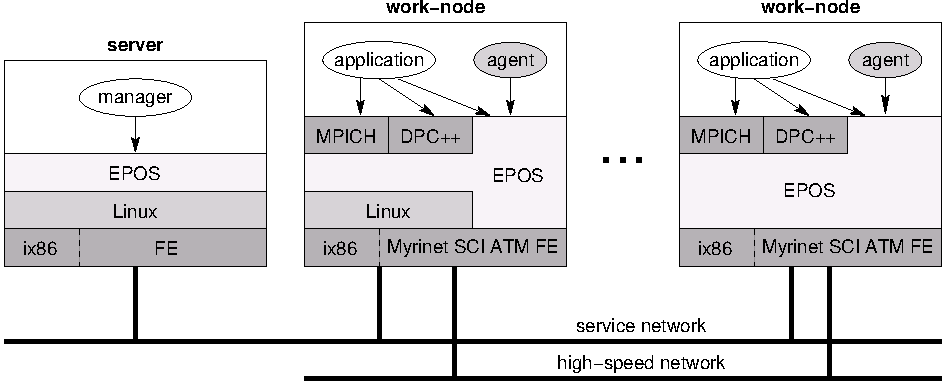
\includegraphics{fig/overview.pdf}}
  \caption{\label{fig:overview}Parallel programming environment overview.}
\end{figure}


\section{Short Bibliography of Project Leaders}

\textbf{Professor Dr. Wolfgang Schr�der-Preikschat} is full professor at
the University of Magdeburg, where he coordinates the Institute for
Distributed Systems. He received a Diplom degree in Computer Science
from the Technical University of Berlin in 1981, and a Ph.D. in Computer
Science from the same university in 1987. His research interests include
embedded, distributed/parallel operating systems, object-oriented
software construction, communication systems, and computer architecture.
\nocite{Buettner:1999}\nocite{Froehlich:sbac:1999}\nocite{Schoen:1998}\nocite{Nolte:1998}\nocite{Preikschat:1994}

\textbf{Professor Dr. Philippe Olivier Alexandre Navaux} is full
professor at the Federal University of Rio Grande do Sul, where he
currently occupies the position of Director of the Institute for
Informatics. He received a B.Sc. in Electric Engineering from the
Federal University of Rio Grande do Sul in 1970, a M.Sc. in Physics from
the same university in 1973, and a Ph.D. in Computer Science from the
Institut National Polytechnique de Grenoble in 1979. His research
interests include computer architecture, operating systems, and parallel
processing.
\nocite{Barreto:1998}\nocite{Cavalheiro:1993}\nocite{Barreto:2000}\nocite{Barreto:2000a}

\textbf{Professor Dr. S�rgio Takeo Kofugi} is assistant professor at the
University of S�o Paulo, where he coordinates the Digital Systems
Division of the Laboratory for Integrated Systems. He received from the
University of S�o Paulo a B.Sc. in Physics in 1981, a M.Sc. in
Electrical Engineering in 1988, and a Ph.D. in Electrical Engineering in
1995. His research interests include high performance computer
architectures and networks.
\nocite{Horta:1998}\nocite{Torres:1997}\nocite{Bernal:1999}

\textbf{Professor Ant�nio Augusto Medeiros Fr�hlich} is assistant
professor at the Federal University of Santa Catarina. He received a
B.Sc. in Computer Science from the Federal University of Rio Grande do
Sul in 1992 and a M.Sc. in Computer Science from the Federal University
of Santa Catarina in 1994. He is currently working towards the Ph.D. at
the Technical University of Berlin.  His research interests include
operating systems and software engineering in the realm of parallel and
embedded computing.
\nocite{Froehlich:sbac:1999}\nocite{Froehlich:ehpc:1999}\nocite{Froehlich:ooosw:1999}\nocite{Froehlich:euromicro:1998}\nocite{Froehlich:intersymp:1996}

%\textbf{Dr. Hans-Georg Paap} is

%\textbf{Engineer Luiz Francisco Gerbase} is one of the founders of ALTUS
%and currently occupies the position of Technology Director. He received
%a M.Sc. in Industrial Electronics from the Federal University of Rio
%Grande do Sul in 1979.


\bibliographystyle{abbrv} 
\bibliography{se,os,network,cluster,guto,snow}

\end{document}

%%% Local Variables: 
%%% mode: latex
%%% TeX-master: t
%%% End: 
